\subsection*{Partie A}

\emph{Pour tout réel $x$, $f(x) = (12x - 480)(x - 10)$.}

$12x - 480 = 0 \iff x = \dfrac{480}{12} = 40$ \quad et \quad $x - 10 = 0 \iff x = 10$.

Les deux coefficients de $x$ (12 et 1) sont positifs : chaque
facteur est négatif avant sa racine et positif après.

\begin{center}
	\begin{tikzpicture}
		\tkzTabInit[lgt=3.4,espcl=2.6]
		{$x$/1,$12x-480$/1,$x-10$/1,$f(x)$/1}{$-\infty$,$10$,$40$,$+\infty$}
		\tkzTabLine{,-,t,-,z,+,}
		\tkzTabLine{,-,z,+,t,+,}
		\tkzTabLine{,+,z,-,z,+,}
	\end{tikzpicture}
\end{center}


\subsection*{Partie B}

\emph{Pour $x \in [0 ; 18]$, $B(x) = 4x^3 - 300x^2 + \np{4800}x - \np{10000}$, où $x$ est le nombre de
tracteurs vendus par mois et $B(x)$ le bénéfice en centaines d'euros.}

\begin{enumerate}
	\item $B(0) = 4 \times 0 - 300 \times 0 + \np{4800} \times 0 - \np{10000} = -\np{10000}$.

	Si l'usine ne vend aucun tracteur dans le mois, elle subit une perte
	de \np{10000} centaines d'euros, soit \np{1000000}~\euro.

	\item Lorsque l'usine vend 18 tracteurs dans le mois, elle réalise un bénéfice de \np{2528}
	centaines d'euros, soit \np{252800}~\euro.

	\item
	\begin{enumerate}
		\item Pour tout réel $x$ de $[0~;~18]$ :
		\[B'(x) = 4 \times 3x^2 - 300 \times 2x + \np{4800} = 12x^2 - 600x + \np{4800}.\]
		D'autre part :
		\[f(x) = (12x - 480)(x - 10) = 12x^2 - 120x - 480x + \np{4800} = 12x^2 - 600x + \np{4800}.\]

Donc, pour tout réel $x$ de $[0 ; 18]$, $B'(x) = f(x)$.

		\item Le signe de $B'(x) = f(x)$ se lit dans le tableau de la partie A, restreint à
		l'intervalle $[0 ; 18]$ : seule la racine 10 s'y trouve ($40 > 18$).

		$B(10) = \np{4000} - \np{30000} + \np{48000} - \np{10000} = \np{12000}$.

		\begin{center}
			\begin{tikzpicture}
				\tkzTabInit[lgt=3.4,espcl=2.8]
				{$x$/1,$B'(x)$/1,$B$/2}{$0$,$10$,$18$}
				\tkzTabLine{,+,z,-,}
				\tkzTabVar{-/$-\np{10000}$,+/$\np{12000}$,-/$\np{2528}$}
			\end{tikzpicture}
		\end{center}

		\item D'après le tableau de variations, $B$ atteint son maximum pour $x = 10$ : l'entreprise
		doit produire et vendre \textbf{10 tracteurs} par mois. Le bénéfice maximal est alors
		$B(10) = \np{12000}$ centaines d'euros, soit \np{1200000}~\euro.
	\end{enumerate}
\end{enumerate}

\medskip
